\section{Résultats}






\begin{minipage}{\linewidth}
    \begin{wrapfigure}{R}{0.5\linewidth}
        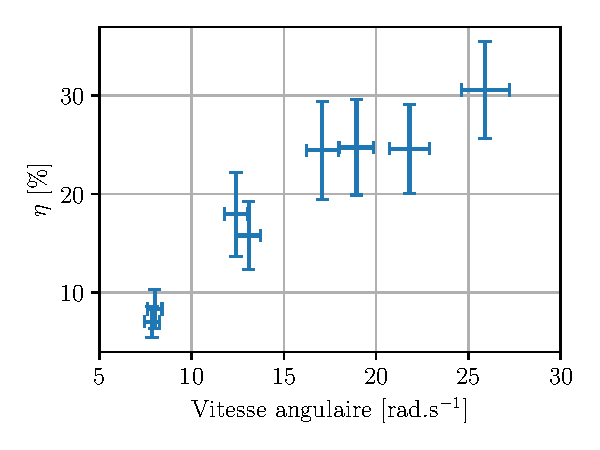
\includegraphics[width=\linewidth]{figures/rend-frigo.pdf}
        \caption{Rendement du cycle frigorifique en fonction du régime de l'arbre de rotation}
        \label{fig:machine_frigo}
    \end{wrapfigure}

    \paragraph*{Rendement du cycle frigorifique}
    Les mesures des puissances du moteur et du filament de compensation permettent un calcul du rendement par l'\autoref{eq:rend-frigo}. La valeur de la température d'équilibre du système entre le refroidissement et la compensation n'a pas été exactement constante sur l'ensemble des mesures mais a tout de même variée de moins de 10 \si{\kelvin}. Les rendements obtenus sont représentés avec leur barre d'erreur en \autoref{fig:machine_frigo}.

\end{minipage}

